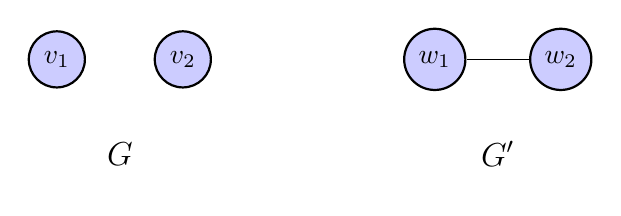
\begin{tikzpicture}  
      [scale=.8,auto=left,every node/.style={circle,fill=blue!20,draw=black,thick}]
      \node (n1) at (0,0) {$v_1$};
      \node (n2) at (2,0) {$v_2$};
      \node (n3) at (6,0) {$w_1$};
      \node (n4) at (8,0) {$w_2$};
      
      \foreach \from/\to in {n3/n4}
      \draw (\from) -- (\to);

      \node[draw=none, fill=none, font=\large] at (1,-1.5) {$G$};
      \node[draw=none, fill=none, font=\large] at (7,-1.5) {$G'$};
\end{tikzpicture}
